\documentclass[
	9pt, % Set the default font size, options include: 8pt, 9pt, 10pt, 11pt, 12pt, 14pt, 17pt, 20pt
	t, % Uncomment to vertically align all slide content to the top of the slide, rather than the default centered
	%aspectratio=169, % Uncomment to set the aspect ratio to a 16:9 ratio which matches the aspect ratio of 1080p and 4K screens and projectors
]{beamer}

\graphicspath{{Images/}{./}} % Specifies where to look for included images (trailing slash required)

\usepackage{booktabs} % Allows the use of \toprule, \midrule and \bottomrule for better rules in tables
\usepackage{graphicx}
\usepackage{caption}
\usepackage{subcaption}
\usepackage{hyperref}
\usepackage[english,brazil]{babel}
\usepackage{fontawesome5}
\usepackage{listings}
\usepackage{minted}
\usepackage{xcolor}
% \usepackage{graphicx}
% \usepackage{animate}
\RequirePackage[backend=biber,
style=ieee,
citestyle=authoryear,
]{biblatex}

% Define a custom command for an icon link
\newcommand{\iconLink}[2]{\href{#1}{\faLink \hspace{0.2em} {#2}}}
\newcommand{\yellowbox}[1]{\colorbox{yellow!75}{#1}}
\definecolor{darkgreen}{rgb}{0,0.5,0}

% Definindo um estilo para o destaque
%----------------------------------------------------------------------------------------
%	SELECT LAYOUT THEME
%----------------------------------------------------------------------------------------
\usetheme{Madrid}

%----------------------------------------------------------------------------------------
%	SELECT COLOR THEME
%----------------------------------------------------------------------------------------

% Beamer comes with a number of color themes that can be applied to any layout theme to change its colors. Uncomment each of these in turn to see how they change the colors of your selected layout theme.

%\usecolortheme{albatross}
%\usecolortheme{beaver}
%\usecolortheme{beetle}
% \usecolortheme{crane}
%\usecolortheme{dolphin}
%\usecolortheme{dove}
%\usecolortheme{fly}
%\usecolortheme{lily}
%\usecolortheme{monarca}
%\usecolortheme{seagull}
%\usecolortheme{seahorse}
%\usecolortheme{spruce}
%\usecolortheme{whale}
%\usecolortheme{wolverine}

%----------------------------------------------------------------------------------------
%	SELECT FONT THEME & FONTS
%----------------------------------------------------------------------------------------
\usefonttheme{default} % Typeset using the default sans serif font

%------------------------------------------------

\usepackage{palatino} % Use the Palatino font for serif text
\usepackage[default]{lato} % Use the Lato font for sans serif text

%----------------------------------------------------------------------------------------
%	SELECT INNER THEME
%----------------------------------------------------------------------------------------
\useinnertheme{rectangles}

%----------------------------------------------------------------------------------------
%	SELECT OUTER THEME
%----------------------------------------------------------------------------------------

% Outer themes change the overall layout of slides, such as: header and footer lines, sidebars and slide titles. Uncomment each theme in turn to see what changes it makes to your presentation.

%\useoutertheme{default}
%\useoutertheme{infolines}
%\useoutertheme{miniframes}
%\useoutertheme{smoothbars}
%\useoutertheme{sidebar}
%\useoutertheme{split}
%\useoutertheme{shadow}
%\useoutertheme{tree}
%\useoutertheme{smoothtree}

%\setbeamertemplate{footline} % Uncomment this line to remove the footer line in all slides
%\setbeamertemplate{footline}[page number] % Uncomment this line to replace the footer line in all slides with a simple slide count

%\setbeamertemplate{navigation symbols}{} % Uncomment this line to remove the navigation symbols from the bottom of all slides

% \bibliography{references} % Specifies the bibliography file to include publications
% \bibliographystyle{apalike} % Specifies the bibliography style
\addbibresource{references.bib}

%----------------------------------------------------------------------------------------
%	PRESENTATION INFORMATION
%----------------------------------------------------------------------------------------

\title[DesWebII]{Desenvolvimento Web II} % The short title in the optional parameter appears at the bottom of every slide, the full title in the main parameter is only on the title page
\subtitle{Aula 08 - Linguagens e frameworks modernos para desenvolvimento web} % Presentation subtitle, remove this command if a subtitle isn't required
\author[Fabricio Bizotto]{Prof. Fabricio Bizotto} % Presenter name(s), the optional parameter can contain a shortened version to appear on the bottom of every slide, while the main parameter will appear on the title slide
\institute[IFC]{Instituto Federal Catarinense \\ \smallskip \textit{fabricio.bizotto@ifc.edu.br}} % Your institution, the optional parameter can be used for the institution shorthand and will appear on the bottom of every slide after author names, while the required parameter is used on the title slide and can include your email address or additional information on separate lines
\date[\today]{Ciência da Computação \\ \today} % Presentation date or conference/meeting name, the optional parameter can contain a shortened version to appear on the bottom of every slide, while the required parameter value is output to the title slide

%----------------------------------------------------------------------------------------
\begin{document}

%----------------------------------------------------------------------------------------
%	TITLE SLIDE
%----------------------------------------------------------------------------------------

\begin{frame}
	\titlepage % Output the title slide, automatically created using the text entered in the PRESENTATION INFORMATION block above
\end{frame}

%----------------------------------------------------------------------------------------
%	TABLE OF CONTENTS SLIDE
%----------------------------------------------------------------------------------------

\begin{frame}
	\frametitle{Roteiro} % Slide title, remove this command for no title
	
	\tableofcontents % Output the table of contents (all sections on one slide)
	%\tableofcontents[pausesections] % Output the table of contents (break sections up across separate slides)
\end{frame}

%----------------------------------------------------------------------------------------
%	PRESENTATION BODY SLIDES
%----------------------------------------------------------------------------------------

\section{Linguagens e frameworks modernos para desenvolvimento web}

\begin{frame}
	\frametitle{Linguagens e frameworks modernos para desenvolvimento web}
	\framesubtitle{O que é framework e para que serve?}

	Um framework é um conjunto de classes e funções que auxiliam o desenvolvimento de um software. Esses códigos trazem funcionalidades já determinadas para agilizar o processo e evitar que as pessoas tenham que reescrever essas funções frequentemente.

	\begin{exampleblock}{Benefícios}
		\begin{itemize}
			\item Agilidade no desenvolvimento
			\item Padronização
			\item Segurança
			\item Manutenção
			\item Comunidade ativa
		\end{itemize}
	\end{exampleblock}

\end{frame}

\begin{frame}
	\frametitle{Linguagens e frameworks modernos para desenvolvimento web}
	\framesubtitle{O que é framework e para que serve?}

	\begin{alertblock}{Desvantagens}
		\begin{itemize}
			\item \textbf{Código Inchado}: muitas vezes o framework traz muitas funcionalidades que não serão utilizadas no projeto.
			\item \textbf{Problemas com suporte}: se o framework não for bem documentado, pode ser difícil encontrar soluções para problemas.
			\item \textbf{Overhead de recursos}: o framework pode consumir muitos recursos do servidor, o que pode ser um problema em projetos com muitos acessos.
		\end{itemize}
	\end{alertblock}

\end{frame}

\begin{frame}
	\frametitle{Linguagens e frameworks modernos para desenvolvimento web}
	\framesubtitle{Principais frameworks para desenvolvimento web}

	\begin{figure}
		\centering
		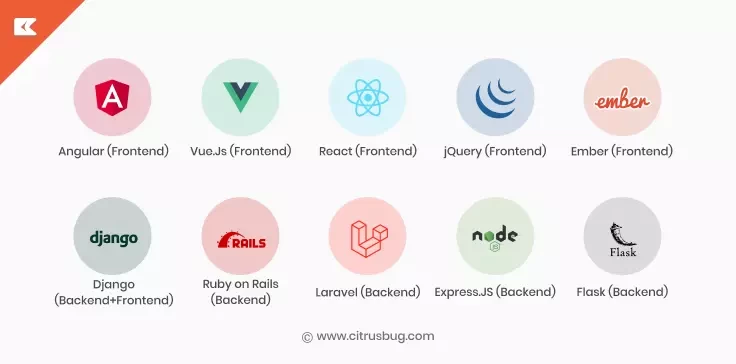
\includegraphics[width=0.9\linewidth]{frameworks_web.png}
		\caption{Principais frameworks para desenvolvimento web}
		\label{fig:frameworks}
	\end{figure}

\end{frame}

\begin{frame}
	\frametitle{Linguagens e frameworks modernos para desenvolvimento web}
	\framesubtitle{JQuery}

	\begin{block}{JQuery}
		\begin{itemize}
			\item Desenvolvido por John Resig em 2006. 
			\item É uma biblioteca JavaScript que facilita a manipulação do DOM, o desenvolvimento de animações e a interação com o servidor.
			\item É uma das bibliotecas JavaScript mais utilizadas no mundo.
			\item Pode ser substituida pela biblioteca \alert{\href{http://vanilla-js.com/}{Vannila JS}}, que é mais leve e performática.
			\item \iconLink{https://jquery.com/}{Site oficial}
		\end{itemize}
	\end{block}

\end{frame}


\begin{frame}
	\frametitle{Linguagens e frameworks modernos para desenvolvimento web}
	\framesubtitle{Angular}

	\begin{block}{Angular}
		\begin{itemize}
			\item Desenvolvido pelo Google em 2010. Popular no desenvolvimento de Single Page Applications (SPA)\footnote{aplicativo web que carrega uma única página HTML e atualiza dinamicamente o conteúdo conforme o usuário interage, proporcionando uma experiência mais fluida e rápida.}.
			\item Utilizava inicialmente a linguagem JavaScript, mas atualmente utiliza TypeScript
			\item Utiliza o padrão de projeto MVC (Model-View-Controller).
			\item Utiliza o conceito de \textbf{two-way data binding}, que permite que a alteração de um elemento na interface reflita automaticamente no modelo de dados e vice-versa.
			\item Usa o conceito de \textbf{diretivas}, que são atributos HTML que permitem a criação de novos elementos HTML.
			\item A partir de 2016, a versão 2 do Angular foi lançada, com grandes mudanças em relação à versão anterior. Atualmente, a versão mais recente é a 17.
			\item \iconLink{https://angular.io/}{Site oficial}
		\end{itemize}
	\end{block}

\end{frame}

\begin{frame}
	\frametitle{Linguagens e frameworks modernos para desenvolvimento web}
	\framesubtitle{React}

	\begin{block}{React}
		\begin{itemize}
			\item Desenvolvido pelo Facebook em 2011. Popular no desenvolvimento de Single Page Applications (SPA).
			\item Utiliza a linguagem JavaScript.
			\item Utiliza o padrão de projeto MVC (Model-View-Controller).
			\item Utiliza o conceito de \textbf{componentes}, que são elementos que encapsulam o código HTML, CSS e JavaScript.
			\item Modernizou a sintaxe do JavaScript, permitindo a manipulação do DOM de forma mais simples.
			\item \iconLink{https://react.dev}{Site oficial}
		\end{itemize}
	\end{block}
\end{frame}

\begin{frame}
	\frametitle{Linguagens e frameworks modernos para desenvolvimento web}
	\framesubtitle{Vue}

	\begin{block}{Vue}
		\begin{itemize}
			\item Desenvolvido por Evan You em 2014. 
			\item Também traz alguns elementos que já comentamos, como data binding, DOM virtual e suporte a SPAs. 
			\item Vue é um framework progressivo que pode ser adotado gradualmente em partes de um projeto, facilitando a integração com projetos existentes.
			\item O ciclo de vida de um componente Vue é composto por 8 etapas: \textbf{beforeCreate}, \textbf{created}, \textbf{beforeMount}, \textbf{mounted}, \textbf{beforeUpdate}, \textbf{updated}, \textbf{beforeDestroy} e \textbf{destroyed}.
			\item Outros frameworks JavaScript: Ember, Backbone, Meteor, Aurelia, Svelte, etc.
			\item \iconLink{https://vuejs.org/}{Site oficial}
		\end{itemize}
	\end{block}

\end{frame}

\begin{frame}
	\frametitle{Linguagens e frameworks modernos para desenvolvimento web}
	\framesubtitle{Ember}

	\begin{block}{Ember}
		\begin{itemize}
			\item Desenvolvido por Yehuda Katz em 2011.
			\item É um framework JavaScript que segue o princípio de \textbf{convenção sobre configuração}. Isso significa que o desenvolvedor não precisa configurar muitas coisas, pois o framework já traz uma série de convenções que facilitam o desenvolvimento.
			\item Utiliza o padrão de projeto MVC (Model-View-Controller).
			\item Usa Handlebars como template engine.
			\item Podemos criar aplicações web completas com Ember, incluindo o backend e Single Page Applications (SPA).
			\item \iconLink{https://emberjs.com/}{Site oficial}
		\end{itemize}

	\end{block}

\end{frame}

\begin{frame}
	\frametitle{Linguagens e frameworks modernos para desenvolvimento web}
	\framesubtitle{Svelte}

	\begin{block}{Svelte}
		\begin{itemize}
			\item Desenvolvido por Rich Harris em 2016.
			\item É um framework JavaScript que utiliza o conceito de \textbf{Build Time Framework}. Isso significa que o código é compilado para JavaScript puro, sem a necessidade de uma biblioteca de terceiros.
			\item \textbf{Zero Runtime:} o código gerado é muito menor do que o código gerado por outros frameworks, o que resulta em uma aplicação mais leve.
			\item \textbf{Programação Declarativa:} o Svelte utiliza uma sintaxe declarativa para a criação de componentes.
			\item Outros frameworks JavaScript: Backbone, Meteor, Aurelia, etc.
			\item \iconLink{https://svelte.dev/}{Site oficial}
		\end{itemize}

	\end{block}

\end{frame}

\begin{frame}
	\frametitle{Linguagens e frameworks modernos para desenvolvimento web}
	\framesubtitle{Next.js}

	\begin{block}{Next.js}
		\begin{itemize}
			\item Desenvolvido por Vercel em 2016.
			\item É um framework JavaScript que utiliza o conceito de \textbf{Server Side Rendering} (SSR). Isso significa que o código é executado no servidor e o HTML é gerado no servidor, o que resulta em uma aplicação mais rápida.
			\item \textbf{Static Site Generation:} o Next.js permite a geração de sites estáticos, o que resulta em uma aplicação mais leve.
			\item \textbf{Roteamento Automático:} as rotas são geradas automaticamente com base na estrutura de pastas do projeto.
			\item \textbf{Hot Module Replacement:} o Next.js permite a atualização de módulos durante o desenvolvimento sem a necessidade de recarregar a página.
			\item Outros frameworks JavaScript: Nuxt.js, Gatsby, Sapper, etc.
			\item \iconLink{https://nextjs.org/}{Site oficial}
		\end{itemize}

	\end{block}

\end{frame}

\begin{frame}
	\frametitle{Linguagens e frameworks modernos para desenvolvimento web}
	\framesubtitle{Laravel}

	\begin{block}{Laravel}
		\begin{itemize}
			\item Desenvolvido por Taylor Otwell em 2011. 
			\item É um framework PHP que utiliza o padrão de projeto MVC (Model-View-Controller).
			\item Possui uma sintaxe simples e elegante, que permite o desenvolvimento de aplicações web de forma rápida e fácil.
			\item Possui uma comunidade ativa e uma documentação completa.
			\item Outros frameworks PHP: Symfony, CodeIgniter, CakePHP, Zend Framework, Yii, Phalcon, FuelPHP, Slim, etc.
			\item \iconLink{https://laravel.com/}{Site oficial}
		\end{itemize}
	\end{block}

\end{frame}

\begin{frame}
	\frametitle{Linguagens e frameworks modernos para desenvolvimento web}
	\framesubtitle{Django}

	\begin{block}{Django}
		\begin{itemize}
			\item Desenvolvido por Adrian Holovaty e Simon Willison em 2003. 
			\item É um framework Python que utiliza o padrão de projeto MVT (Model-View-Template).
			\item Pode ser usado para criar uma aplicação com backend e frontend, ou apenas o backend (API).
			\item Outros frameworks Python: Flask, Pyramid, Bottle, CherryPy, Tornado, etc.
			\item \iconLink{https://www.djangoproject.com/}{Site oficial}
		\end{itemize}
	\end{block}

\end{frame}

\begin{frame}
	\frametitle{Linguagens e frameworks modernos para desenvolvimento web}
	\framesubtitle{Spring}

	\begin{block}{Spring}
		\begin{itemize}
			\item Desenvolvido por Rod Johnson em 2002. 
			\item É um framework Java que utiliza o padrão de projeto MVC (Model-View-Controller).
			\item Usa Gradle ou Maven para gerenciar dependências.
			\item Outros frameworks Java: JSF, Struts, Vaadin, GWT, Wicket, Hibernate, JPA, Maven, etc.
			\item \iconLink{https://spring.io/}{Site oficial}
		\end{itemize}
	\end{block}

\end{frame}

\begin{frame}
	\frametitle{Linguagens e frameworks modernos para desenvolvimento web}
	\framesubtitle{Ruby on Rails}

	\begin{block}{Ruby on Rails}
		\begin{itemize}
			\item Desenvolvido por David Heinemeier Hansson em 2004. 
			\item É um framework Ruby que utiliza o padrão de projeto MVC (Model-View-Controller).
			\item Possui uma sintaxe simples e elegante, que permite o desenvolvimento de aplicações web de forma rápida e fácil.
			\item Possui uma comunidade ativa e uma documentação completa.
			\item Outros frameworks Ruby: Sinatra, Padrino, Hanami, Devise, etc.
			\item \iconLink{https://rubyonrails.org/}{Site oficial}
		\end{itemize}
	\end{block}

\end{frame}

\begin{frame}
	\frametitle{Linguagens e frameworks modernos para desenvolvimento web}
	\framesubtitle{Express}

	\begin{block}{Express}
		\begin{itemize}
			\item Desenvolvido por TJ Holowaychuk em 2010. 
			\item É um framework JavaScript que utiliza o padrão de projeto MVC (Model-View-Controller).
			\item É um dos frameworks mais populares para desenvolvimento de aplicações web com Node.js.
			\item Outros frameworks Node.js: Koa, Hapi, Sails, Meteor, Nest, etc.
			\item \iconLink{https://expressjs.com/}{Site oficial}
		\end{itemize}
	\end{block}

\end{frame}

\begin{frame}
	\frametitle{Linguagens e frameworks modernos para desenvolvimento web}
	\framesubtitle{ASP.NET}

	\begin{block}{ASP.NET}
		\begin{itemize}
			\item Desenvolvido pela Microsoft em 2002. 
			\item É um framework que utiliza o padrão de projeto MVC (Model-View-Controller).
			\item É um dos frameworks mais populares para desenvolvimento de aplicações web com .NET.
			\item Outros frameworks .NET: ASP.NET Core, Nancy, ServiceStack, etc.
			\item \iconLink{https://dotnet.microsoft.com/apps/aspnet}{Site oficial}
		\end{itemize}
	\end{block}

\end{frame}

\begin{frame}
	\frametitle{Linguagens e frameworks modernos para desenvolvimento web}
	\framesubtitle{Considerações finais}

	\begin{block}{Considerações finais}
		\begin{itemize}
			\item A escolha de um framework depende do tipo de aplicação que será desenvolvida, da linguagem de programação que será utilizada, do conhecimento da equipe, do tempo disponível para o desenvolvimento, entre outros fatores.
			\item A escolha de um framework deve ser feita com cuidado, pois uma vez que o projeto é iniciado com um framework, é difícil mudar para outro.
			\item A escolha de um framework deve ser feita com base em critérios técnicos, e não apenas por modismo ou por ser o mais popular.
		\end{itemize}
	\end{block}

\end{frame}

\section{Experimentos}

\begin{frame}
	\frametitle{Experimentos}
	\framesubtitle{Atividade prática}

	\begin{enumerate}
		\item Pesquise sobre frameworks web e escolha um deles para estudar.
		\item Crie um repositório no GitHub
		\item Crie um arquivo README.md com as informações sobre o framework escolhido, contendo: {\small \textbf{Nome do framework, Ano de lançamento, Desenvolvedor, Linguagem de programação, Padrão de projeto utilizado, Quando é recomendado utilizar o framework, Principais características (mínimo de 3), Um vídeo, podcast ou artigo sobre o framework, Site oficial}}.
		\item Compartilhe o link do repositório com um colega e peça para ele revisar o seu arquivo README.md
		\item Faça a revisão do arquivo README.md do seu colega e dê sugestões de melhoria via pull request.
		\item Crie um exemplo prático de uso do framework escolhido e compartilhe no repositório. Pode ser uma aplicação web simples para:
		\begin{itemize}
			\item Manipulação do DOM, Consumo de uma API, Criação de um componente, etc
			\item Converter texto para voz
			\item Sistema de votação para uma enquete em tempo real
			\item Outra funcionalidade que você achar interessante
		\end{itemize}
		\item Compartilhe novamente o link do repositório com o colega e peça para ele revisar o seu exemplo prático.
		\item \textbf{Encerramento}: reflexão em grupo sobre a experiência.
	\end{enumerate}

\end{frame}


\end{document} 
